\chapter{Indledning}
Behovet for intelligent hjælp i hjemmet er voksende. Særligt bevægelseshæmmede mennesker - som mennesker, der lider af ALS - har et stort behov for hjælp, men det er dyrt at have personale ansat til at hjælpe dem. \\ 
Hjælpeenheder til handicappede er også dyre at anskaffe, og begrænser sig ofte til én enkelt funktion. Med EyeRobot skal det være slut med disse begrænsninger.

Den lille hjælpende robot styres med øjnene, så selv personer med ALS vil føle begrænsningerne for den fysiske bevægelighed blive lettet. 
Robotten sender samtidigt videofeed tilbage, så brugeren kan se, hvad den laver, uanset hvor den er.

EyeRobots software skal installeres på brugerens computer, og kræver kun et webcam. \\
På grund af EyeRobots universal port, kan den let udbygges med mange forskellige moduler, så den kan tilpasset den enkelte brugers behov, uden at brugeren skal betale for funktionalitet han/hun ikke har brug for. 
Hvis du eksempelvis har brug for en ekstra arm, så kan der nemt tilkobles en robot-arm til EyeRobot \cite{moscow}.

Figur \ref{fig:Rigt_billede} viser EyeRobots koncept.

\begin{figure}[tbph]
	\centering
	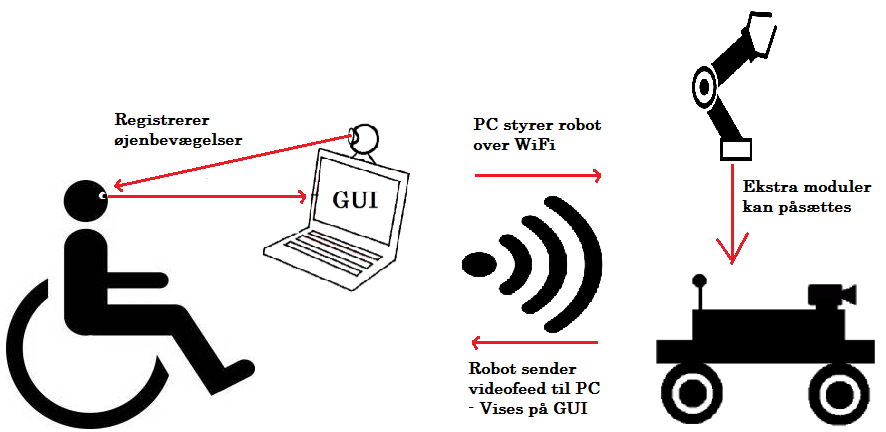
\includegraphics[width = \textwidth]{figur/Rigt_billede.png}
	\caption{Konceptuelt billede af EyeRobot}
	\label{fig:Rigt_billede}
\end{figure}